Kubernetes là một hệ thống mã nguồn mở để quản lý và triển khai ứng dụng có độ linh hoạt cao trên môi trường đám mây và trung tâm dữ liệu. Được phát triển bởi Google và sau đó chuyển giao cho Cloud Native Computing Foundation (CNCF), Kubernetes đã trở thành một trong những công cụ quản lý container phổ biến nhất trong ngành công nghiệp Công nghệ Thông tin.\cite{k8s-doc}

Với mục tiêu chính là tự động hóa quy trình triển khai, mở rộng và quản lý ứng dụng container, Kubernetes giúp giảm thiểu gánh nặng cho các nhà phát triển và quản trị hệ thống. Hệ thống này cung cấp một nền tảng đồng nhất cho việc triển khai, mở rộng và quản lý ứng dụng container trên nhiều máy chủ.

Mô hình làm việc của Kubernetes tập trung vào các đối tượng như Pod, Service, ReplicaSet, và nhiều khái niệm khác, tạo ra một môi trường linh hoạt cho triển khai và quản lý ứng dụng. Điều này giúp các nhà phát triển xây dựng ứng dụng một cách dễ dàng và nhà quản trị hệ thống duy trì chúng một cách hiệu quả.

Kubernetes không chỉ hỗ trợ các mô hình triển khai truyền thống mà còn tạo ra cơ hội cho các chiến lược mới như Continuous Deployment (CD - liên tục triển khai phần mềm) và Microservices. Với khả năng tự động hóa nhiều khía cạnh của quy trình phát triển và triển khai ứng dụng, Kubernetes đóng vai trò quan trọng trong việc xây dựng và duy trì các hệ thống phức tạp, linh hoạt và có khả năng mở rộng.

\subsection{Giới thiệu một số khái niệm}

Kubernetes đưa ra một loạt các khái niệm quan trọng để quản lý và triển khai ứng dụng, cung cấp một môi trường linh hoạt và hiệu quả. Dưới đây là một giới thiệu về các khái niệm chính của Kubernetes: Pod, ReplicaSet, Deployment và Service.

\begin{figure}[H]
    \centering
    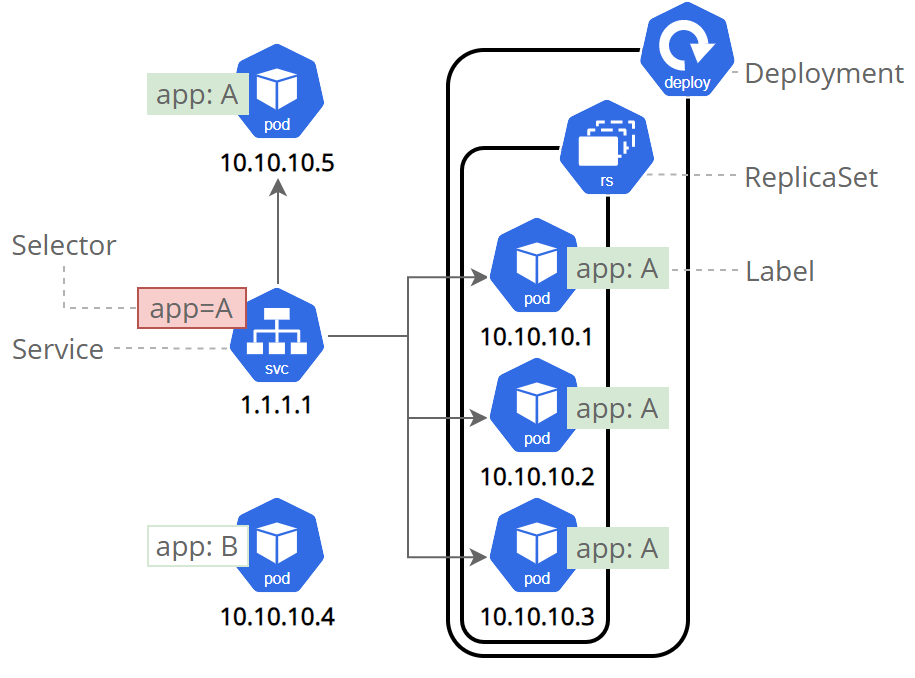
\includegraphics[width=0.75\linewidth]{Images/3.4-k8s-comps.png}
    \caption{Tổng quan về Kubernetes - Kubernetes}
    \label{fig:k8s-comps}
\end{figure}

\begin{itemize}
    \item \textbf{Pod}: là đơn vị cơ bản nhất trong Kubernetes, đại diện cho một nhóm các container chia sẻ một không gian làm việc. Các container trong cùng một Pod chia sẻ mạng và lưu trữ, giúp chúng tương tác và làm việc cùng nhau. \\
    Pod cung cấp một môi trường chung cho các container, giúp chúng kết hợp để tạo thành các ứng dụng có độ phức tạp cao.

    \item \textbf{ReplicaSet}: là một tài nguyên trong Kubernetes dùng để đảm bảo rằng một số lượng xác định các Pod đang chạy theo cách nhất định. Nếu một Pod bị lỗi hoặc tắt, ReplicaSet sẽ tự động khởi chạy một Pod mới để thay thế. \\
    ReplicaSet giúp duy trì trạng thái ổn định của ứng dụng bằng cách đảm bảo rằng một số lượng nhất định của các Pod luôn tồn tại và hoạt động.

    \item \textbf{Deployment}: quản lý quá trình triển khai và cập nhật ứng dụng trong Kubernetes. Nó định nghĩa trạng thái mong muốn của ứng dụng và đảm bảo rằng ReplicaSet được cập nhật để đạt được trạng thái đó. \\
    Deployment cung cấp khả năng quản lý linh hoạt, cho phép triển khai phiên bản mới, hạ cấp, và thậm chí rollback đối với ứng dụng mà không gây gián đoạn dịch vụ.

    \item \textbf{Service}: là một tài nguyên trong Kubernetes giúp cung cấp một HTTP port vào các Pod. Nó tạo ra một địa chỉ IP và tên DNS duy nhất cho một nhóm các Pod, giúp các ứng dụng giao tiếp với nhau và với bên ngoài. \\
    Service giúp ẩn đi sự phức tạp của việc quản lý nhiều Pod và địa chỉ IP, cung cấp một cách dễ dàng và liền mạch để truy cập các dịch vụ trong môi trường Kubernetes.
\end{itemize}

\subsection{Ưu - nhược điểm}
Thông thường, các hệ thống lớn thường áp dụng Kubernetes trong quá trình phát triển và triển khai các sản phẩm phần mềm của họ. Điều này có thể mang đến một số lợi lớn như:
\begin{enumerate}
    \item Quản lý tài nguyên hiệu quả: Với khả năng quản lý tài nguyên chặt chẽ, Kubernetes giúp tối ưu hóa việc sử dụng tài nguyên máy chủ và container, đảm bảo hiệu suất tối ưu và giảm lãng phí.
    \item Khả năng tự hồi phục: Trong quá trình vận hành, các service thường có nguy cơ gặp sự cố. Kubernetes sẽ tự động khắc phục các sự cố trong tình huống này nhằm đảm bảo tính sẵn sàng cao (High-Availability).
\end{enumerate}

Tuy nhiên, việc công nghệ vẫn có một số điểm yếu. Bao gồm:
\begin{enumerate}
    \item Độ phức tạp cao: Với những người mới bắt đầu, đây là một trong những công nghệ cực kỳ khó để tiếp cận. Người học cần nắm vững rất nhiều loại kiến thức khác nhau: Mạng máy tính, containerization, ...
    \item Yêu cầu về tài nguyên: Triển khai và duy trì Kubernetes đòi hỏi một số lượng tài nguyên đáng kể, bao gồm cả nhân sự và phần cứng, đặc biệt là đối với các tổ chức nhỏ.
\end{enumerate}
